\section{Distribuzione delle variabili}
In questo capitolo si è analizzata la distribuzione per ogni singola variabile [\ref{fig:distrubution_1}] e la distribuzione della singola variabile dividendo i valori assunti in base alle due classi [\ref{fig:distrubution_2}], ovvero vino di bassa qualità e vino di alta qualità.

\noindent
Per ogni grafico sull'asse delle ordinate si trova il range di valori assunti dalle istanze nel dataset mentre sull'asse delle ascisse si trova la stima di densità di probabilità.

\noindent
La densità di probabilità si può vedere come quanta possibilità ho di avere un determinato valore considerando la classe e/o la variabile; inoltre la rappresentazione di questo valore astrae dalla numerosità di un determinato tipo di istanze.

\noindent
Questo tipo di grafico può avere problemi con valori non continui, ma tenderà a mantenere una curva morbida anche con valori discreti e con valori mancanti.

\noindent
Questa è un'analisi univariata, ovvero viene considerata una singola variabile alla volta, osserveremo solo una variabile per ogni grafico presentato in questo capitolo.

\noindent
Non verranno prese in considerazione le relazioni tra diverse variabili, ma si cercherà di descrivere aspetti della singola variabile anche rispetto alle classe di qualità.

\noindent
Il grafico delle distribuzioni permette di capire i valori che i dati tendono ad assumere, si può notare se assumono valori secondo una distribuzione standard oppure se tendono ad assumere maggiormente valori in alcuni specifici range, si può anche capire se sono presenti valori anomali.

\noindent
Considerando anche le classi è possibile notare quanto i dati delle due classi sono correlati e la differenza tra le due distribuzioni.

\noindent
Se una variabile tende ad avere due distribuzioni molto differenti per forma o per valori assunti allora si può pensare che la variabile rappresentata dal determinato grafico possa essere utile per distinguere le due classi di qualità.

\noindent
Questo aspetto è particolarmente utile nelle fasi successive, infatti può influire sull'analisi delle componenti principali, sul modello di classificazione e anche sull'analisi dei risultati ottenuti dai modelli.

\begin{figure}[H]
    \centering
    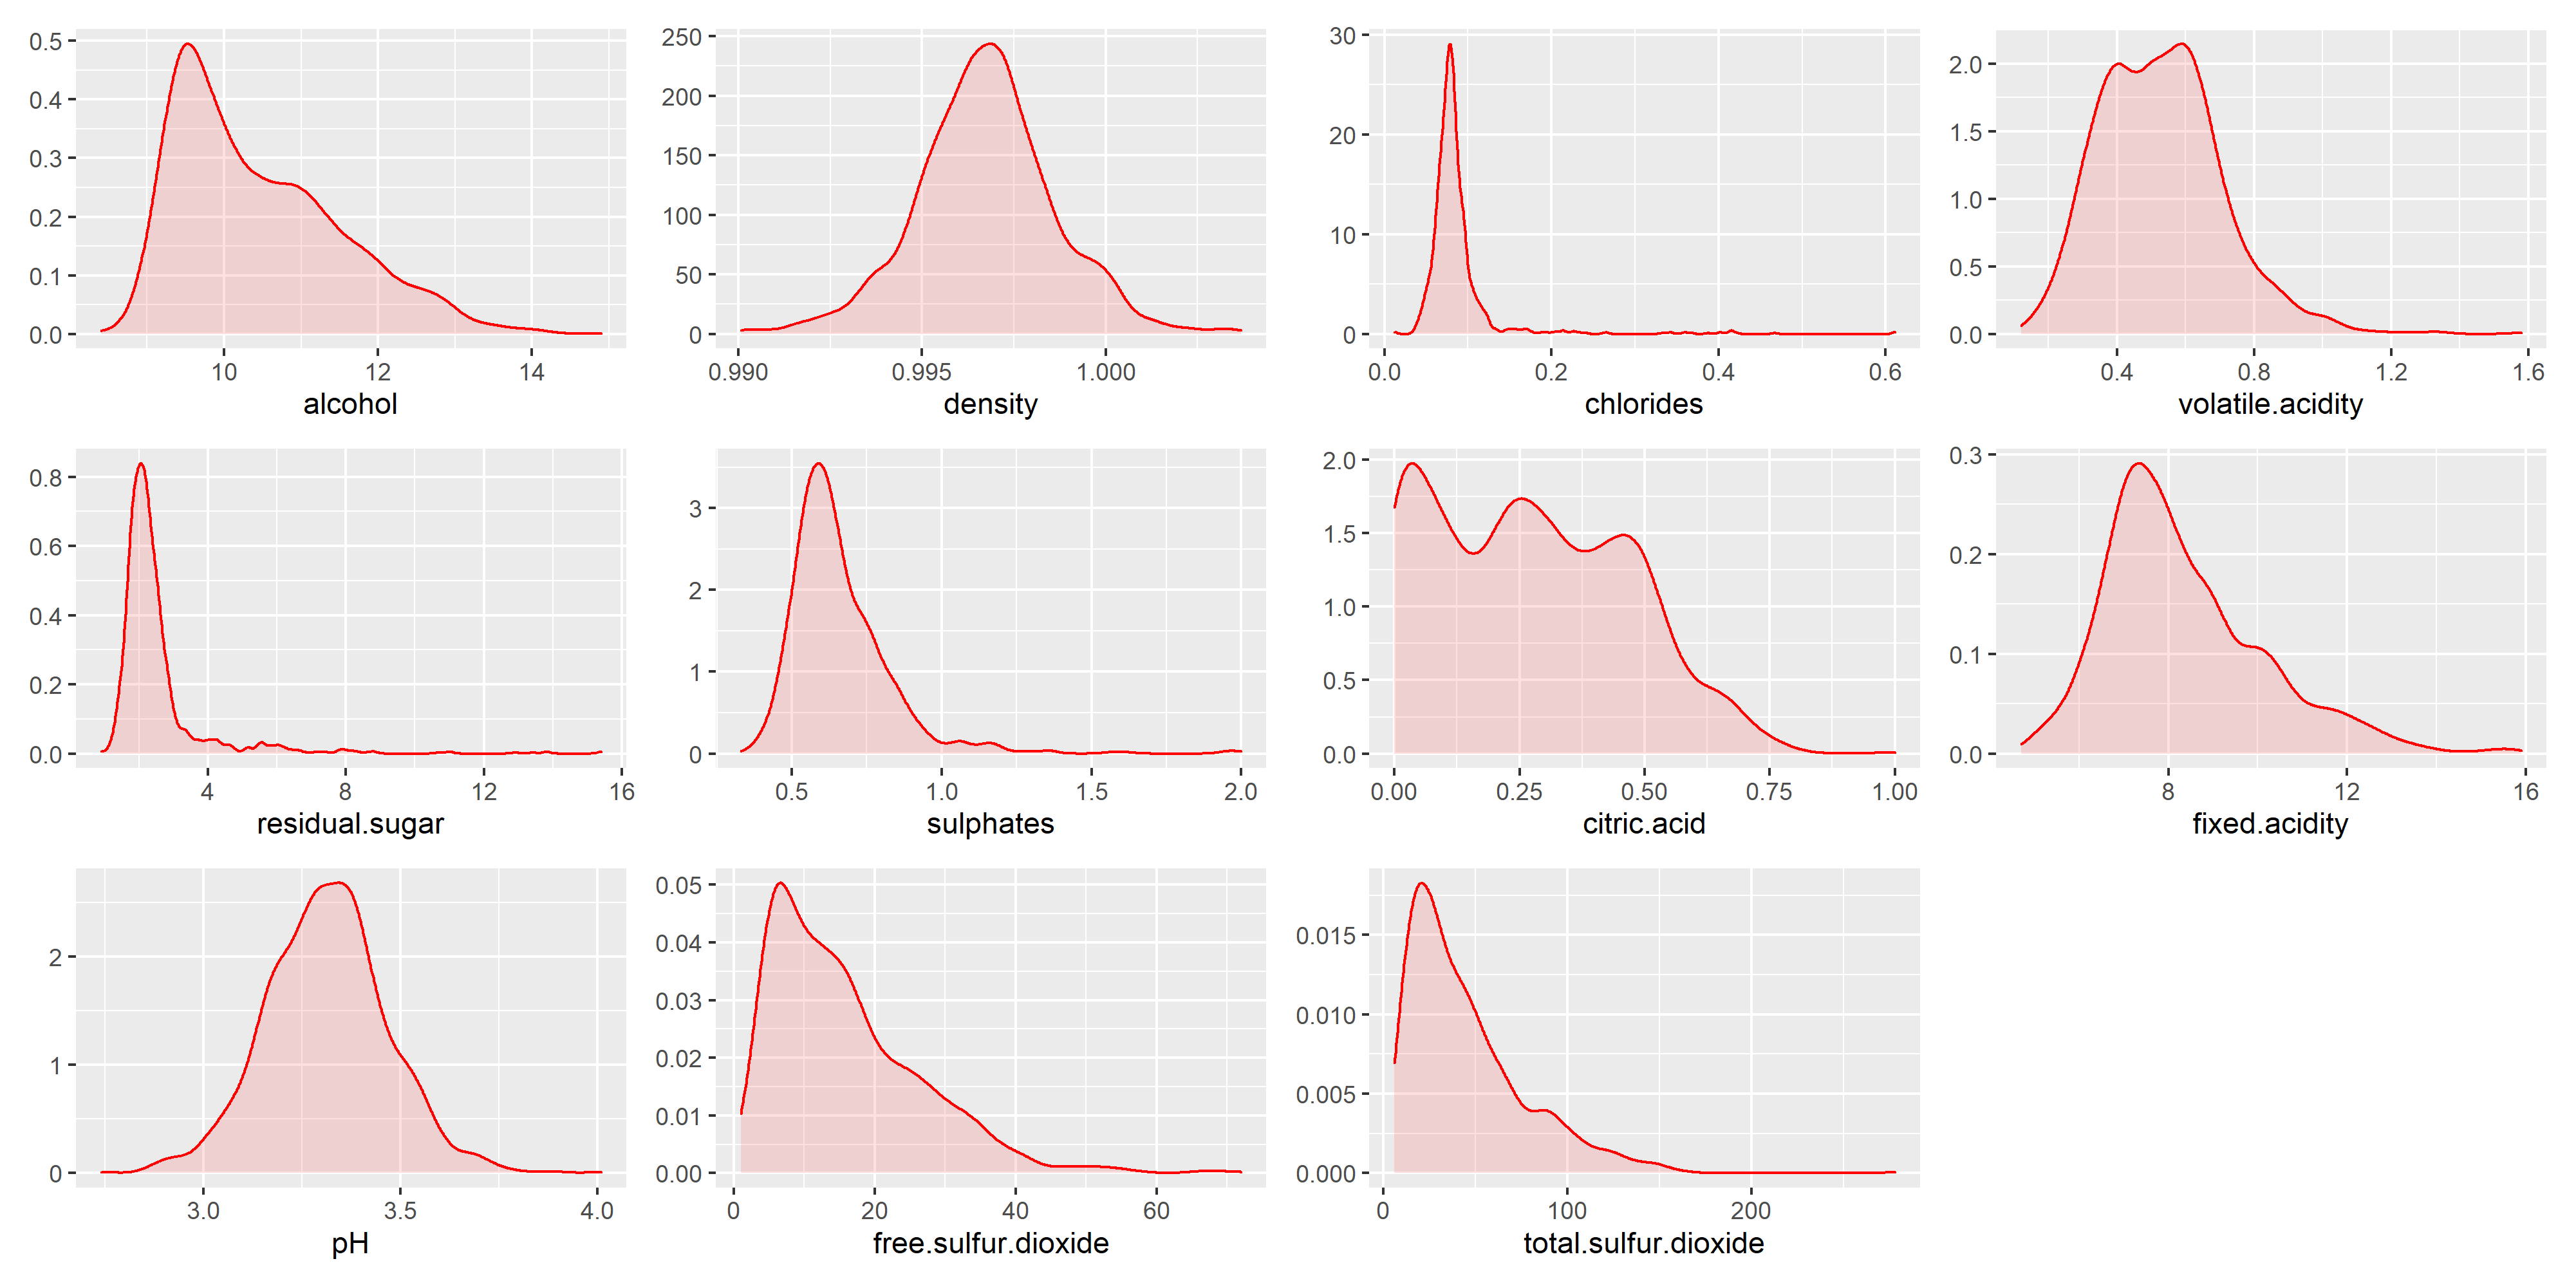
\includegraphics[width=\linewidth]{images/analisi/distribuzioni_variabili/distribution1.png}
    \caption{Questa immagine consiste in un insieme di grafici, dove ogni singolo grafico rappresenta la distribuzione dei valori assunti da una specifica variabile.}
    \label{fig:distrubution_1}
\end{figure}

\begin{figure}[H]
    \centering
    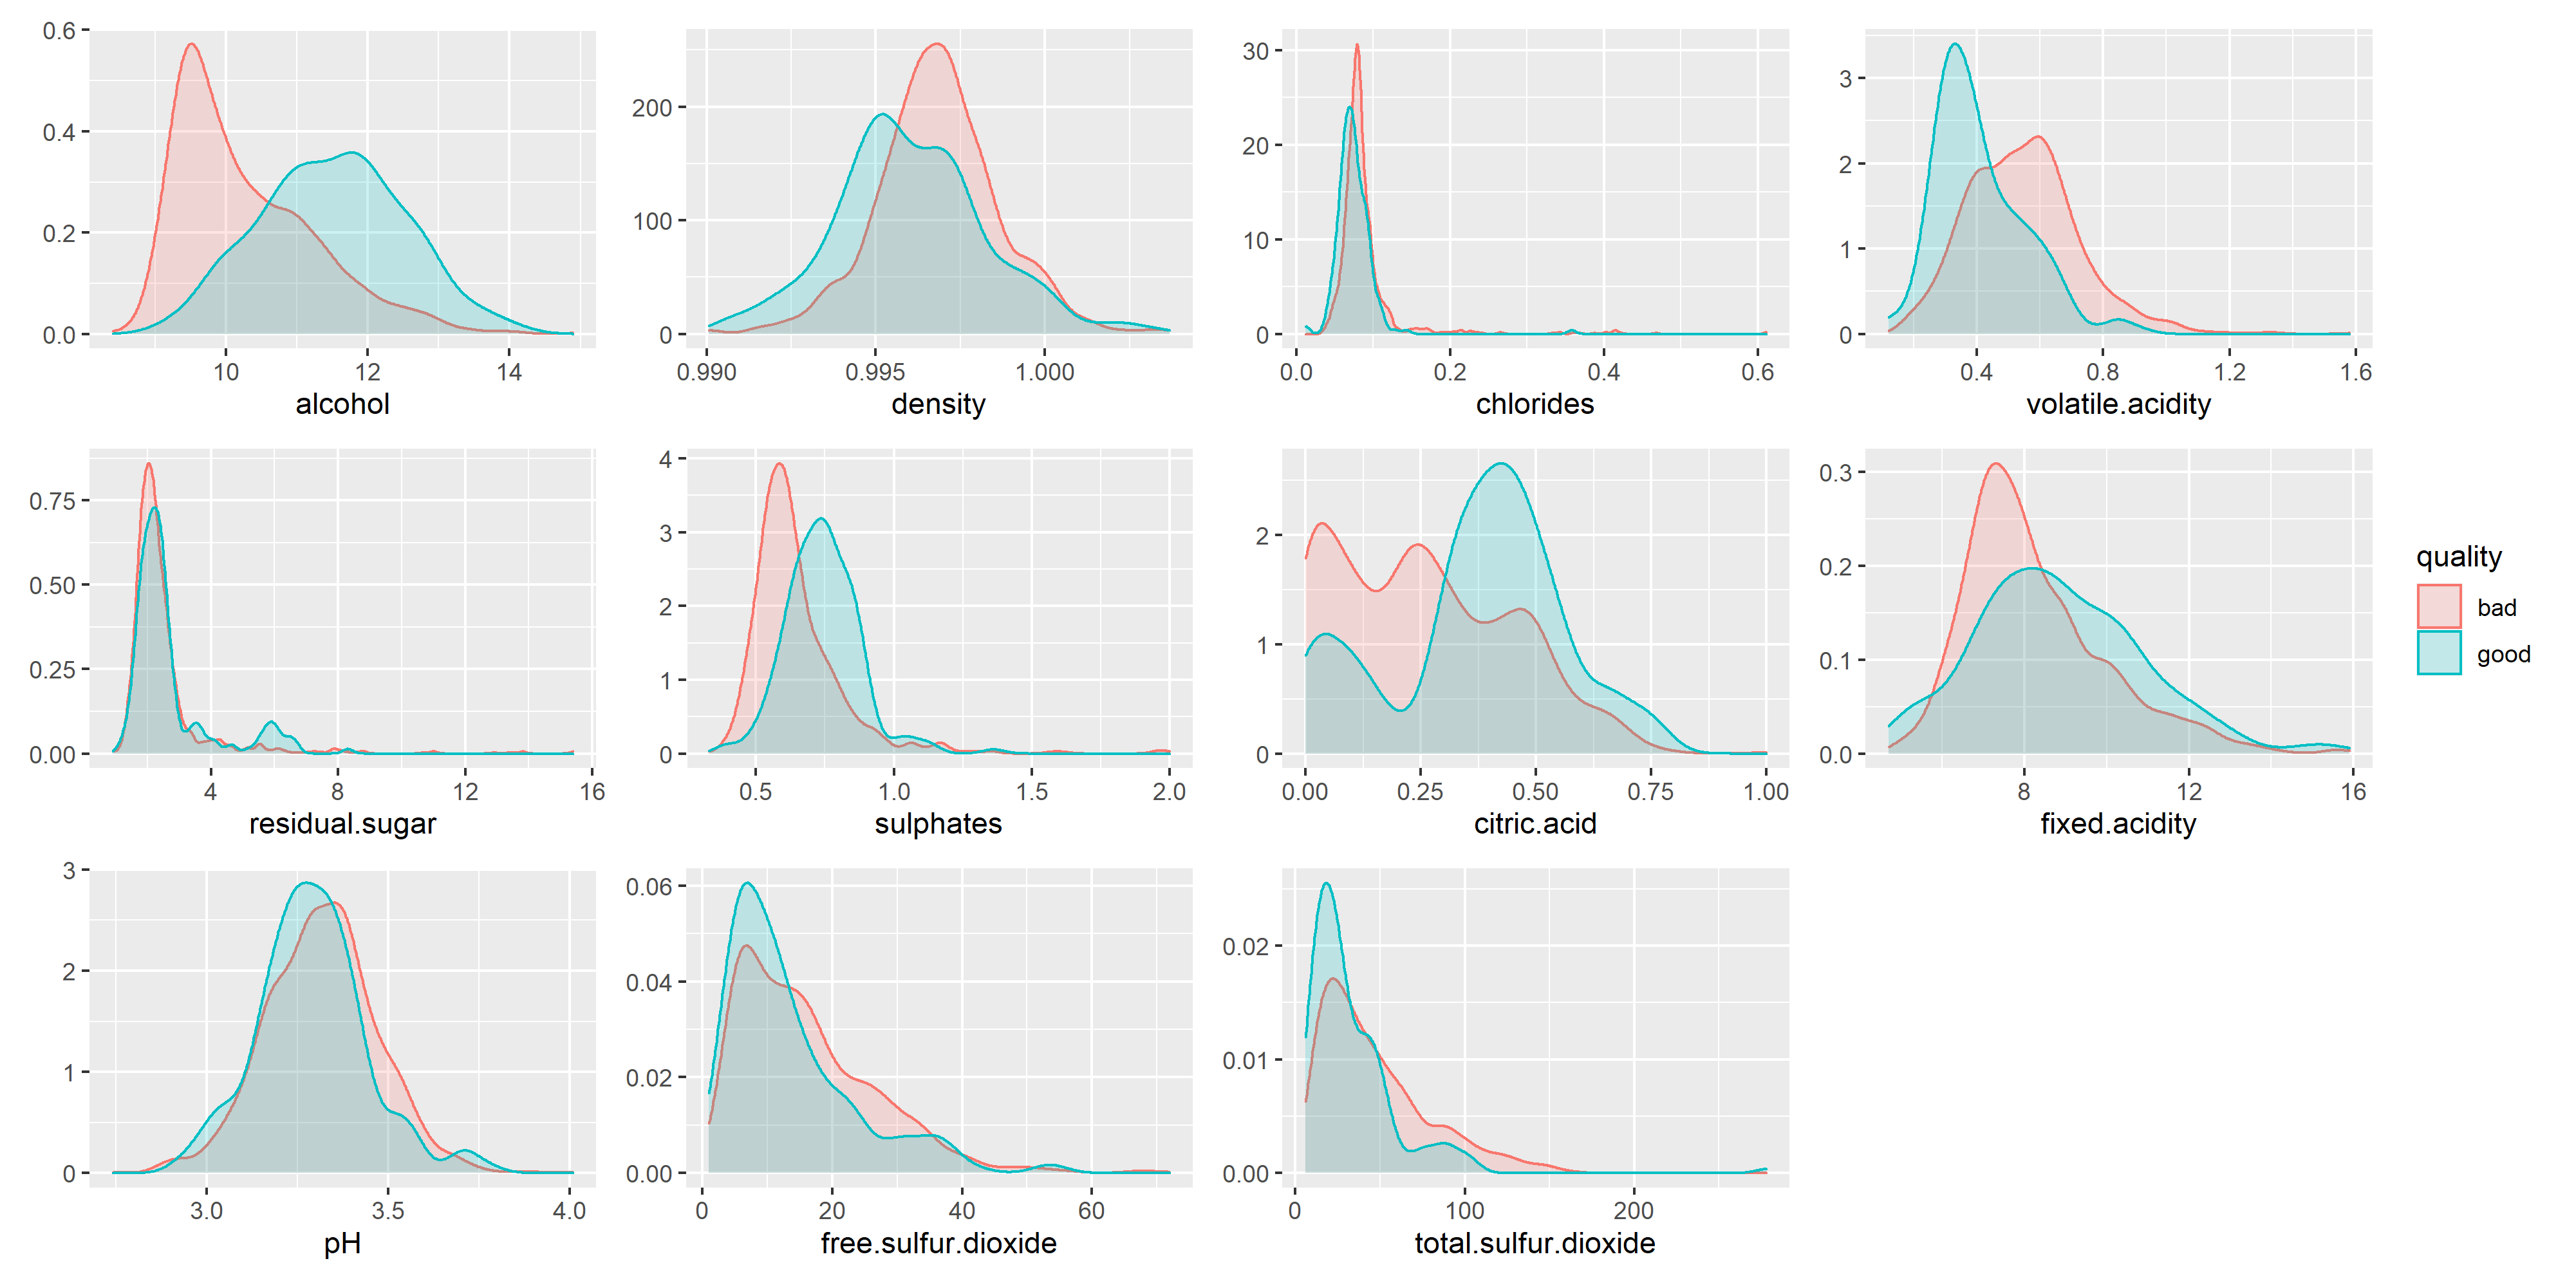
\includegraphics[width=\linewidth]{images/analisi/distribuzioni_variabili/distribution2.png}
    \caption{Questa immagine consiste in un insieme di grafici, dove ogni singolo grafico rappresenta la distribuzione dei valori assunti da una specifica variabile mettendo in evidenza la classe ($bad$ e $good$) a cui appartengono.}
    \label{fig:distrubution_2}
\end{figure}

\noindent
Dai grafici [\ref{fig:distrubution_1}] e [\ref{fig:distrubution_2}] si può notare come soltanto la variabile \textit{alcohol} abbia delle sostanziali differenze tra le due distribuzioni delle due classi e questo la rende molto interessante.

\newpage

\noindent
Le altre variabili tendono a non caratterizzare la differenza tra le due classi se non in minima parte. Questo indica la complessità presente nel distinguere le due classi per un possibile modello.

\noindent
Questa scarsa caratterizzazione rispecchia le difficoltà, già descritte nell'introduzione [\ref{ch:introduzione}], che si trovano nel produrre e nello svolgere le analisi.
